\section{Epilogue: A theory for elliptic loci in the confocal pair}

%The affine transformation  $x\rightarrow{x/a}$, $y\rightarrow{y/b}$ sends the confocal pair to a pair where the outer conic is the unit circle and the caustic $\E_c'$ is a concentric ellipse. The foci $f,g$ of the $\E_c'$ are given by:

%\[ f=(-c',0),\;\;\;g=(c',0) \]

%\noindent where $c'=(1/c)\sqrt{2 \delta -a^2-b^2}$.

\begin{proposition}
If a triangle center $X_k$ is stationary over a Poncelet 3-periodic family, then the locus of any triangle center $\X$ which is a fixed linear combination of $X_2,X_3,X_k$ will be an ellipse. 
\label{prop:07-fixed-lin-comb}
\end{proposition}

\begin{proof}
The triangle center $\X=\alpha X_2+ \beta X_3+ \gamma X_k$ is the linear combination $\X\ab:=\alpha X_2+ \beta X_3$ under a fixed translation by $\gamma X_k$, because both $\gamma X_k$ and $X_k$ are fixed over the family.
\end{proof}

This entails the most compact rendition of the following result (appearing originally in \cite{helman2021-theory}:

\begin{corollary}
Over billiard 3-periodics, the locus of $X_1$ is an ellipse.
\label{cor:07-x1-ellipse}
\end{corollary}

\begin{proof}
For any triangle, $X_1$ can be expressed as the linear combination $X_1=\alpha X_2+\beta X_3+\gamma X_9$ of $X_2$, $X_3$ and $X_9$ with:

\[ \alpha =\frac{6}{\rho+2},\;\;\beta=\frac{2\rho}{\rho+2},\;\;\gamma=\frac{-\rho-4}{\rho+2} \]

\noindent where $\rho=r/R$, is the ratio of inradius to circumradius. Since in the confocal family $X_9$ is stationary and $\rho$ is invariant \cite{reznik2020-intelligencer}, the claim follows.
\end{proof}

Table \cref{tab:07-x1-methods} shows a history of proof techniques of the ellipticity of $X_1$ over billiard 3-periodics:

\begin{table}
\begin{tabular}{|l|c|l|l|}
\hline
Author & Year & Technique  & Reference \\
\hline
D. Reznik        & 2011 & Experimental Video &  \cite{reznik2011-incenter} \\
O. Romaskevich   & 2014 & Complex Analytic  Geometry  &  \cite{olga14}  \\
R. Garcia        & 2016 & Real Analytic   Geometry &  \cite{ garcia2019-incenter}  \\
(in this book)   & 2021 & Specialize $X_1$ locus to confocal pair &  \cref{cor:07-X1q2}  \\
M. Helman et al. & 2021 & 3-Center Linear Combination  &  \cite{helman2021-theory} \\
\hline
\end{tabular}
\caption{Various proof methods for the ellipticity of $X_1$ over billiard 3-periodics.}
\label{tab:07-x1-methods}
\end{table}

We can expand the above result to other triangle centers in the confocal pair, as many of these are fixed linear combinations of $X_2$, $X_3$, and $X_9$. 

\begin{proposition}
In the confocal pair, from $X_1$ to $X_{200}$, the loci of $X_k$ are ellipses, $k=$1,  2,  3,  4,  5,  7,  8,  10,  11,  12,  20,  21,  35,  36,  40,  46,  55,  56,  57,  63,  65,  72,  78,  79,  80,  88$^\dagger$, 84,  90, 100, 104, 119, 140, 142, 144, 145, 149, 153, 162$^\dagger$, 165, 190$^\dagger$, 191, 200.
\end{proposition}

\begin{proof}
As in the previous corollary, one can write $X_1$ as a fixed linear combination of $X_2$, $X_3$, and $X_9$, given that the ratio $\rho=r/R$ is constant in the confocal pair.
In \cite[Table 2
]{helman2021-theory}, a table of fixed coefficients $\alpha,\beta,\gamma$ is provided expressing each of the triangle centers in the claim as fixed linear combinations of $X_1$, $X_2$ and $X_3$. \cref{tab:07-abg} reproduces those results. Therefore all triangle centers in the claim (except for $X_{88}$, $X_{162}$, and $X_{190}$) are fixed linear combinations of $X_1$, $X_2$, and $X_3$, and therefore they are fixed linear combinations of $X_2$, $X_3$, and $X_9$ as well. By \cref{prop:07-fixed-lin-comb}, given that $X_9$ is stationary over the confocal family, this implies the loci of all these triangle centers are ellipses.
\end{proof}

$^\dagger$Note: the loci of $X_{88}$, $X_{162}$, and $X_{190}$ (called ``swans'' before) are also ellipses because by definition they lie on the circumconic centered on $X_9$ \cite[X(9)]{etc}.

\begin{table}
\begin{minipage}{2.0in}
\begin{tabular}{|c|c|c|c|}
\hline
$X_k$ & $\alpha$ & $\beta$ & $\gamma$ \\
\hline$X_1$ &$1$ & $0$ & $0$ \\
$X_2$ & $0$ & $1$ & $0$  \\
$X_3$ & $0$ & $0$ & $1$  \\
$X_4$ & $0$ & $3$ & $-2$ \\
$X_5$ & $0$ & $3$ & $-1$ \\
$X_{7}$ & $\frac{2\rho+4}{\rho+4}$ & $\frac{3\rho}{\rho+4}$ & $\frac{-4\rho}{\rho+4}$  \\
$X_9$ & $\frac{-\rho-2}{\rho+4}$ & $\frac{6}{\rho+4}$ & $\frac{2\rho}{\rho+4}$\\
$X_{10}$ & $1$ & $-3$ & $0$  \\
$X_{11}$ & $\frac{1}{1-2\rho}$ & $\frac{-3\rho}{1-2\rho}$ &  $\frac{\rho}{1-2\rho}$  \\ 
$X_{12}$ & $\frac{1}{1+2\rho}$ & $\frac{3\rho}{1+2\rho}$ &  $\frac{-\rho}{1+2\rho}$  \\ 
$X_{20}$ & $0$ & $3$ & $-4$ \\
$X_{21}$ & $0$ & $\frac{3}{2\rho+3}$ & $\frac{2\rho}{2\rho+3}$  \\
$X_{35}$ & $\frac{1}{2\rho+1}$ &  $0$ & $\frac{2\rho}{2\rho+1}$ \\
$X_{36}$ & $\frac{1}{1-2\rho}$ & $0$ & $\frac{-2\rho}{1-2\rho}$  \\
$X_{40}$ & $1$ & $0$ & $-2$ \\
$X_{46}$ & $\frac{1+\rho}{1-\rho}$ & $0$ & $\frac{-2\rho}{1-\rho}$ \\
$X_{55}$ & $\frac{1}{1+\rho}$ & $0$ & $\frac{\rho}{1+\rho}$  \\
$X_{56}$ & $\frac{1}{1-\rho}$ & $0$ & $\frac{-\rho}{1-\rho}$ \\
$X_{57}$ & $\frac{2+\rho}{2-\rho}$ & $0$ & $\frac{-2\rho}{2-\rho}$  \\
$X_{63}$ & $\frac{-\rho-2}{\rho+1}$ & $\frac{3}{\rho+1}$ &  $\frac{2\rho}{\rho+1}$\\
\hline
\end{tabular}
\end{minipage}
\begin{minipage}{2.0in}
\begin{tabular}{|c|c|c|c|}
\hline
$X_k$ & $\alpha$ & $\beta$ & $\gamma$ \\
\hline
$X_{65}$ & $\rho+1$ & $0$ & $-\rho$ \\ 
$X_{72}$ & $-\rho-2$ & $3$ & $\rho$ \\
$X_{78}$ & $\frac{\rho+2}{\rho-1}$ & $\frac{-3}{\rho-1}$ & $0$ \\ 
$X_{79}$ & 1 & $\frac{6\rho}{2\rho+3}$ & $\frac{-6\rho}{2\rho+3}$ \\ 
$X_{80}$ & $\frac{2\rho+1}{-2\rho+1}$ & $\frac{-6\rho}{-2\rho+1}$ &  $\frac{2\rho}{-2\rho+1}$ \\
$X_{84}$ & $\frac{-\rho-2}{\rho}$ & $\frac{6}{\rho}$ & $\frac{2\rho-4}{\rho}$ \\ 
$X_{90}$ & $\frac{-(\rho+1)^2}{\rho^2+2\rho-1}$ & $\frac{6\rho}{\rho^2+2\rho-1}$ & $\frac{2\rho(\rho-1)}{\rho^2+2\rho-1}$\\ 
$X_{100}$ & $\frac{2}{2\rho-1}$ & $\frac{-3}{2\rho-1}$ & $\frac{2\rho}{2\rho-1}$ \\
$X_{104}$ & $\frac{-2}{2\rho-1}$ & $\frac{3}{2\rho-1}$ & $\frac{2\rho-2}{2\rho-1}$ \\ 
$X_{119}$ & $\frac{1}{2\rho-1}$ & $\frac{3\rho-3}{2\rho-1}$ & $\frac{-\rho+1}{2\rho-1}$ \\
$X_{140}$ & $0$ & $3$ & $1$  \\
$X_{142}$ & $\frac{\rho+2}{2\rho+8}$ & $\frac{3\rho+6}{2\rho+8}$ & $\frac{-2\rho}{2\rho+8}$ \\
$X_{144}$ & $\frac{4\rho+8}{-\rho-4}$ & $\frac{3\rho-12}{-\rho-4}$ & $\frac{-8\rho}{-\rho-4}$\\
$X_{145}$ & $4$ & $3$ & $0$ \\
$X_{149}$ & $\frac{-4}{6\rho-3}$ &  $\frac{9-6\rho}{6\rho-3}$ &  $\frac{12\rho-8}{6\rho-3}$ \\
$X_{153}$ & $\frac{4}{6\rho-3}$ & $\frac{-6\rho-3}{6\rho-3}$ & $\frac{12\rho-4}{6\rho-3}$ \\
$X_{165}$ & $1$ & $0$ & $-4$ \\
$X_{191}$ & $-1$ & $\frac{6}{2\rho+3}$ & $\frac{4\rho}{2\rho+3}$ \\
$X_{200}$ & $\frac{\rho+4}{\rho-2}$ & $\frac{-6}{\rho-2}$ & $0$ \\
\hline
\end{tabular}
\end{minipage}
\caption{Coefficients $\alpha,\beta,\gamma$ used to express $X_k$ as the linear combinations $\alpha X_1+\beta X_2+\gamma X_3$. Note: $\rho=r/R$. Note also that although though the loci of $X_{88}$, $X_{162}$, and $X_{190}$ are ellipses (they sweep the elliptic billiard), they are cannot be expressed fixed linear combinations of $X_1,X_2,X_3$. Notice $\alpha$,$\beta$,$\gamma$ are the same up to sign of $\rho$ for harmonic conjugate pairs ($X_{11}$,$X_{12}$), ($X_{35}$,$X_{36}$), ($X_{55}$,$X_{56}$).}
\label{tab:07-abg}
\end{table}

Referring to \cref{fig:07-confocal-degenerate}:

\begin{proposition}
In the confocal pair, the locus of $\X=\alpha X_2+\beta X_3$ for $\alpha,\beta\in\R$ is a circle when:

\[\left(\frac{\alpha}{\beta}\right)_{\pm}=\frac{\delta-3 a b\pm 2\left(a^2+b^2\right)}{2 a b} \]
\end{proposition}

\begin{proof}
By \cref{lem:ell-param}, this will happen when $|u|+|v|=\big||u|-|v|\big|$ with $u,v$ from \cref{thm:07-ellipse-locus}. In the confocal pair, when $\alpha,\beta\in\R$, both $u$ and $v$ are real numbers as well. Thus, this condition holds if and only if either $u=0$ or $v=0$. The ratios $\alpha/\beta$ that yield circular loci can then be computed directly.
\end{proof}

\begin{observation}
It follows that $\left({\alpha}/{\beta}\right)_+ +\left({\alpha}/{\beta}\right)_-=-3$.
\end{observation}

\begin{definition}[Degenerate Locus] When the elliptic locus of a triangle center is a segment, i.e., one of its axes has shrunk to zero, we will call it ``degenerate''.
\end{definition}

\begin{proposition}
Let $\X$ be a fixed linear combination of $X_2$, $X_3$, and $X_k$, where $X_k$ is some stationary center over the family of 3-periodics. As the vertices of the 3-periodics sweep the outer ellipse monotonically, the path of $\X$ in its elliptical locus is monotonic as well, except for when this locus is degenerate.
\end{proposition}

\begin{proof}
By \cref{thm:07-ellipse-locus}, the locus of $\X$ can be parametrized by $u \l+v\frac{1}{\l}+w$ for some $u,v,w\in\mathbb{C}$, where $\l$ sweeps the unit circle in $\mathbb{C}$ in the same direction as the 3-periodic vertices sweep the outer ellipse of the Poncelet pair. We can thus parametrize $\X$ as $\X(t)=u e^{i t}+v e^{-i t}+w$. If either $u=0$ or $v=0$, it is clear from this parametrization that $\X$ sweeps its locus monotonically. Thus, we can now assume that $u\neq0$ and $v\neq0$.

Denoting $u=u_0+i u_1$ and $v=v_0+i v_1$ with $u_0,u_1,v_0,v_1\in\R$, we can directly compute
\[
    \left|\frac{d}{d t}\X(t)\right|^2= |u|^2+|v|^2 + 2 \sin (2 t) (u_2 v_1-u_1 v_2)-2 \cos (2 t) (u_1 v_1+u_2 v_2)
\]

Since $(u_2 v_1-u_1 v_2)^2+(u_1 v_1+u_2 v_2)^2=(u_1^2+u_2^2)(v_1^2+v_2^2)=|u|^2|v|^2$, there is some angle $\phi\in[0,2\pi)$ (the angle between the vectors $(u_1,u_2)$ and $(v_1,v_2)$) such that $u_1 v_1+u_2 v_2=|u| |v|\cos\phi$ and $u_2 v_1-u_1 v_2=|u| |v|\sin\phi$. Substituting this back in the previous equation, we derive
\begin{gather*}
     \left|\frac{d}{d t}\X(t)\right|^2=|u| |v|\left(\frac{|u|}{|v|}+\frac{|v|}{|u|}+2\sin(2t)\sin(\phi)-2\cos(2t)\cos(\phi)\right)=\\
     =|u| |v|\left(\frac{|u|}{|v|}+\frac{|v|}{|u|}-2\cos(2t+\phi)\right)\geq |u| |v|\left(\frac{|u|}{|v|}+\frac{|v|}{|u|}-2\right)
\end{gather*}

By AM-GM inequality, this last quantity is always strictly greater than 0 unless $|u|=|v|$. If $|u|\neq|v|$, we will have $\left|\frac{d}{d t}\X(t)\right|^2>0$, and hence the velocity vector never vanishes, meaning that the $\X$ sweeps its smooth locus monotonically. By \cref{lem:ell-param}, this means that $\X$ sweeps its locus monotonically except when this locus is degenerate.

\end{proof}

\begin{figure}
    \centering
    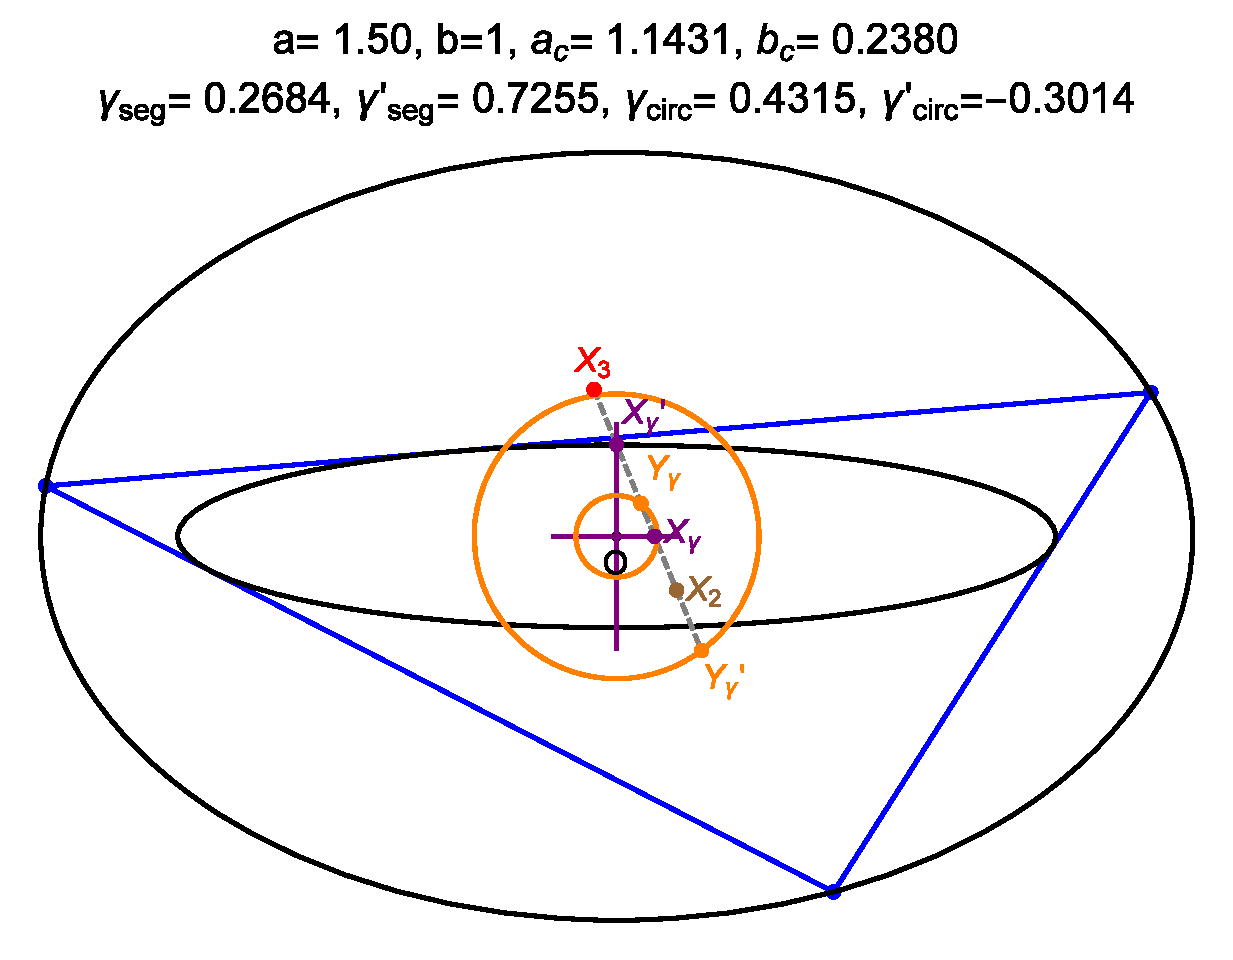
\includegraphics[width=.7\textwidth]{pics_07_060_confocal_degenerate_circle_gammas}
    \caption{A 3-periodic (blue) in a pair of confocal ellipses (black) with $a/b=1.5$. Also shown are two degenerate (segment-like) loci (purple) obtained with $\gamma{\simeq}\{.27,.73\}$ and two circular loci (orange), obtained with $\gamma{\simeq}\{.43,-.3\}$. \href{https://youtu.be/haFTsq5UyK4}{Video}}
    \label{fig:07-confocal-degenerate}
\end{figure}

In \cref{sec:05-triple-winding} we provided a continuity argument for the three turns executed by a triangle center over a traversal of the billiard 3-periodic family.

\begin{remark}
In \cite[Lemma 3.4, p. 28]{daepp-2019} it is shown that (i) the complex argument of the Blaschke product is monotonic on the unit circle, and that (ii) for each $\lambda$ there are 3 solutions for the equation $B(z)=\lambda$. This means that as $\lambda$ sweeps the unit circle monotonically, the 3-periodics sweep the outer Poncelet ellipse monotonically and in the same direction as $\lambda$. Moreover for every 3 full cycles of $\lambda$ over the complex the unit circle, each vertex of the 3-periodics sweep the outer ellipse exactly once.
\label{rem:monotone-Blaschke}
\end{remark}

\begin{proposition}
Let $\X$ be a fixed linear combination of $X_2$, $X_3$, and $X_k$, where $X_k$ is some stationary center over the family of 3-periodics. Over a full cycle of 3-periodics, the winding number of $\X$ over its elliptical locus is $\pm 3$, except for when this locus is degenerate.
\end{proposition}



\begin{proof}
By \cref{thm:07-ellipse-locus}, the locus of $\X$ can be parametrized by $u \l+v\frac{1}{\l}+w$ for some $u,v,w\in\mathbb{C}$. From \cref{rem:monotone-Blaschke}, one can see that the winding number of $\lambda$ associated to 3-periodics is $+3$ for each full cycle of 3-periodics over the outer Poncelet ellipse. Thus, it is sufficient to prove that the winding number of $\X$ over its elliptical locus is $\pm 1$ as $\lambda$ goes around the complex unit circle just once.

Since $w$ is the center of the elliptic locus of $\X$ (see \cref{lem:ell-param}), we compute the winding number of $\X$ around $w$. Parametrizing $\X$ as $\X(t)=u e^{i t}+v e^{-i t}+w$ where $\lambda=e^{i t}$, one can directly compute the winding number as \cite[Lemma 1, p. 114]{ahlfors1979-complex}:

\[
    \frac{1}{2\pi i}\oint_{\X}\frac{d\zeta}{\zeta-w}=\frac{1}{2\pi i}\int_0^{2\pi} \frac{\X'(t)}{\X(t)-w}d t={\mathop{\mathrm{sign}}}(|u|^2-|v|^2)
\]

By \cref{lem:ell-param}, the only way we can have $|u|=|v|$ is if the locus of $\X$ is degenerate. Thus, whenever this locus is not degenerate, the winding number of $\X$ around its locus as $\lambda$ sweeps the unit circle once is equal to $1$ if $|u|>|v|$ and $-1$ when $|u|<|v|$, as desired.
\end{proof}